\subsection{2-2 RunThreeToEight}

\subsubsection*{Code}

\inputgroovy[label=CreateSetsOfEight.groovy,firstline=4]{../ChapterExercises/src/c2/CreateSetsOfEight.groovy}
\inputgroovy[label=GenerateSetsOfThree.groovy,firstline=4]{../ChapterExercises/src/c2/GenerateSetsOfThree.groovy}
\inputgroovy[label=ListToStream.groovy,firstline=4]{../ChapterExercises/src/c2/ListToStream.groovy}
\inputgroovy[label=RunThreeToEight.groovy,firstline=5]{../ChapterExercises/src/c2/RunThreeToEight.groovy}

\subsubsection*{Results}

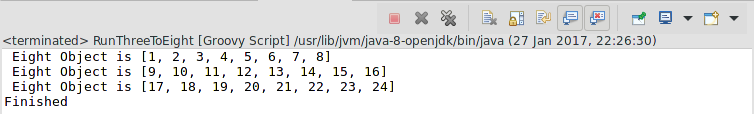
\includegraphics[width=\textwidth]{img/screenshots/2-2.png}


\subsubsection*{Questions}

\paragraph{1. What change is required to output objects containing six integers?}

To update the code to generate groups of 6 instead of 8 we can change the for loop in {\em CreateSetsOfEight.groovy} from \mintinline{groovy}{for ( int i in 0 .. 7 )} to \mintinline{groovy}{for ( int i in 0 .. 5 )}.

\paragraph{2. How could you parameterise this in the system to output objects that contain any number of integers (e.g. 2, 4, 8, 12) ?}

To parameterise the solution to any group size we can add a groupSize parameter to the output list generator.

\inputgroovy[label=CreateSetsParameterised.groovy,firstline=4]{../ChapterExercises/src/c2/CreateSetsParameterised.groovy}
\inputgroovy[label=RunThreeToAny.groovy,firstline=5]{../ChapterExercises/src/c2/RunThreeToAny.groovy}


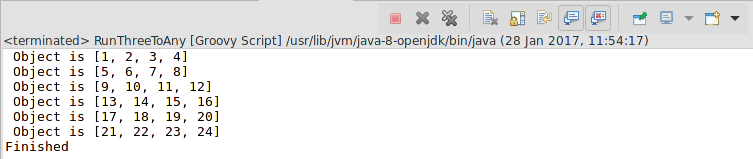
\includegraphics[width=\textwidth]{img/screenshots/2-2-q2.png}

\paragraph{3. What happens if the number of integers required in the output stream is not a factor of the total number of integers in the input stream (e.g. 5 or 7) ?}

If the output groupSize is not a factor of the total number of input integers the system will print out as many full groups as it can make and then freeze without completing or printing the semi created group.

This is because, in {\em CreateSetsParameterised }, the while loop \mintinline{groovy}{ while( v != -1) } is only checked on completion of the for loop \mintinline{groovy}{ for ( i in 1 .. groupSize ) }.  If the groupSize parameter is not a factor of the total input number then this for loop never completes, as the program gets stuck trying to read from \mintinline{groovy}{ inChannel }.  If this for loop never finishes, the program can never complete.

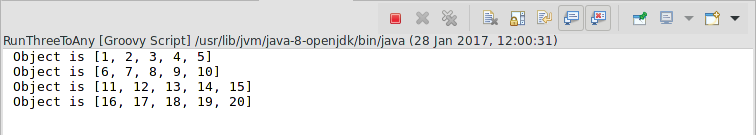
\includegraphics[width=\textwidth]{img/screenshots/2-2-q3.png}
